%%\documentclass[referee,sn-basic]{sn-jnl}% referee option is meant for double line spacing
%%\documentclass[lineno,sn-basic]{sn-jnl}% Basic Springer Nature Reference Style/Chemistry Reference Style

\documentclass[default,pdflatex,iicol]{sn-jnl}% Default with double column layout

%%<additional latex packages if required can be included here>
\usepackage[numbers]{natbib}

\jyear{2021}
\raggedbottom
%%\unnumbered% uncomment this for unnumbered level heads

\begin{document}

\title[Article Title]{Nearcam Tapline Detection 2}

\author[]{\fnm{Rattachai} \sur{Wongtanawijit}}\email{rattachai.gov@gmail.com}
\equalcont{These authors contributed equally to this work.}

\author*[*]{\fnm{Thanate} \sur{Khaorapapong}}\email{thanate.khao@gmail.com}
\equalcont{These authors contributed equally to this work.}

\affil*[1]{\orgdiv{Department of Computer Engineering, Faculty of Engineering}, \orgname{Prince of Songkla University}, \orgaddress{\street{P.O. Box 2 Kohong}, \city{HatYai, Songkhla}, \postcode{90112}, \country{Thailand}}}

\abstract{Current image-task-related convolutional neural network structures lean toward the directed acyclic graph that allows multiple output nodes. This enables a solution for the rubber tapping line detection that various desired output types, such as bounding boxes, pixel points or edges, are necessary. This paper demonstates that such deep networks with their outputs are bounding box and semantic pixel segmenation mask by adopting YOLO and U-Net layer structures. This paper proposes a column-wise argmax function with the technique of redundant mask outputs intended to enhance pixel classification accuracy. Experiments with the networks discover that some novel segmentation loss functions have different characters for tapping line prediction which were observed with geometric distance and F1-score. The redundant mask output can omits their weaknesses and yield higher detection accuracy compare to every single ones. Also, the column-wise argmax well suit to the tapping line detection in place of a thinning algorithm rather than the thresholding on the spatial output neurons.}

\keywords{\textit{hevea brasiliensis}, Semantic Edge, Rubber Tapping, Tapping Line, YOLO}

\maketitle

%% Section
\section{Introduction}\label{sec-introduction}

A self-instructed robot that has abilities to detect things and interact with, a sensory device with a detection algorithm is at least required. The detail of a vision system of a rubber tapping robot by a robotic arm, e.g. \cite{patent1, patent2, patent3, WANG2022103906}, which introduced in \cite{Wongtanawijit_2021}, adopted a near-range camera co-operating with specifically designed algorithm to perform tapping line detection. Continuing on the previous work, this paper presents another tapping line detection algoirthm in a whole different way. Given the definition of a tapping line in an image, is a piecewise polynomial where its vertices are at the pixels in the image grid \cite{Wongtanawijit_2021}. The detection is to precisely locate that pixels.

Motivations of this paper come from recent deep convolutional neural nets (CNN), such as object bounding-box detector, mask, edge-aware or semantic edge segmentation networks. But, none of them are ready-to-use solution for this problem. Original contributors of those works designed their networks to fit into more generic data than the tapping line images. This encourages this paper to explore other researches that answer how can those generic networks be adopted for some more specific datasets that might be useful for the tapping line detection.

Considering the essences of CNN-based object detectors architectures, many of them shared some common properties such as layer configurations. For example, the downstream convolution path shrinks down the input's spatial dimensions. In any arbitary layer orders, high-level detection which known as "classification" happens in low-resolution tensors, while other lower semantics such as edge detection are performed at higher tensor's resolution. This is because individual parts in CNN play the different roles. Some layers extract the useful information, while others shape that information to the desire outputs which specified by the loss functions. Notable differences are at the network's output or head. A box detector's output is the grid coordinates which represent the location and the dimension of the boxes, while the output of segmentation mask is the probability score at each pixels.

For the tapping line, this paper demonstates a network that composed of multiple different output types. Box outputs roughly determine where the tapping line is in a rectangular area. Pixel classification output answers where the polyline's vertices are wihtin the box. Network's structure are arranged in a directed acyclic graph in order to make the network trainable with gradient-based back-propagation optimizer with the end-to-end training scheme. A pixel classification head obtains the data from the downsampling-upsampling path likewise in U-Net \cite{unet}, V-Net \cite{vnet} or other pixel-level segmentation networks. Co-operating with the proposed column-wise argmax function, the networks can directly produce tapping lines without any post-processings. The network calculates the boxes' coordinates at two prediction heads with the earlier YOLO \cite{redmonyolov2} 's regression form.

Training to detect tapping lines, a set of novel loss for pixel classfication on very unbalanced data, Dice-Coefficient, Binary Focal, and Tversky indices are inspected for loss-value convergence and the prediction accuracy. The overall loss for the network is the combination of YOLO's box regression and pixel classification losses. Assessing the network's performance, a set of evaluation metrics are applied to the predictions. The Intersection-Over-Union (IoU) ratios of the box clearify the existence of a tapping line in an image. F1-score and distance errors describe the closeness of the predicted pixels to the actual tapping line inside the box.

Detection results appear to be diverse when the network are trained with different pixel classification loss. There are some trade-off between F1-score and Hausdorff distance, but all is on par with each others. Every models provide above 92.0 percents in average precisions with bounding box evaluation. The results also point that by the appending of column-wise Softmax to the pixel prediction head helps the networks to gain more accuracy than the widely used pixel-wise activated neurons. 

In order to archieve the higher detection accuracy, this paper also presents a modification in top layers of pixel classification head for separately predict multiple loss or deep supervising, then gather all of them by voting for the pixel majorities with the use of column-wise Softmax function. The proposed method can generate the results in higher F1-score with also diminishes the distance between two polylines.

The rests of this paper include: the review of literatures in Section \ref{sec-review} \textemdash e.g. the previous work of the tapping line detection, relevant applications of muliple output node CNN detectors, etc. The design of tapping line detection network in Section 3. The experiment setup and results in Section 4 and Section 5. Summary with the disscussions are in Section 6.

\section{Background and Motivation}\label{sec-background}
The purpose of the near-range vision camera is for precisely locate the tapping position for tapping manipulation of the robot arm. Our previous work \cite{Wongtanawijit_2021} demonstrated the detection algorithm in a form of an image processing algorithm. The method produces accurate results but it was specially designed and required two input images accommodating by artificial lighting patterns for the nighttime farming. Apart from this paper that, the CNN-based detectors can learn what and where is the tapping line under any lighting circumstance depends on the training dataset. Moreover, tappling line detection by modern computer vision algorithms is not yet explored at this time. Hence, it is a interesting topic to study the capable of CNN-based detectors with the tappline line image dataset, and might be useful as an alternate algorithm for the robot.

%% Section
\section{Review of Literatures}\label{sec-review}
\subsection{Tapping Line Detection}
Rubber tapping is a process of farming the natural rubber latex from a Pará rubber tree (\textit{Hevea brasiliensis}). Tapping is making a cut on the rubber tree bark or the tapping panel letting the latex to flow along. This cut is leaving a gutter that called the tapping path. Refer to the rubber tapping document \cite{abraham1992tapping}, the cut is recommended to be 30 to 45 degrees angle to the ground axis. Likewise, small angle tolerances are acceptable. A robot with a robot arm integrated, which able to do tapping automatically, probably have been installed a close-up camera for fine detail acquisition as in many visual-servoing systems (patents \cite{patent1, patent2, patent3}). Consequently, the appearance of a tapping path is a certain line in the image which named the "tapping line".

The image data with labels are necessary for developing a machine learning algorithm by the supervised learning. Previous tapping line detection work \cite{Wongtanawijit_2021} labels a tapping line by two annotations. A bounding box encodes the tapping endpoints that to be at the top-left and the bottom-right corner of the box. Then, a polyline or a piecewise polynomial connect two endpoints. As a results, the polyline's vertices can be defined on every columns inside the box in order to simplify the annotations.

\subsection{Overview of Deep Convolutional Neural Networks}
The developments of core ideas on deep CNN-based detectors quite become settled in last 5 years. Back then when CNN-based box detectors, Faster-RCNN \cite{fasterrcnn} and YOLO \cite{redmonyolov1}, were established in 2015. Much more recent detectors such as YOLOv3 \cite{redmonyolov3} (2018), YOLOv4 \cite{alexyyolov4} (2020) able to detect any objects in the images with such very high rates than their predecessors. Later researches put lots of improvements on the modern networks. For some details, YOLOv3 and v4 have multiple prediction head that works on different spatial resolution so that the detector better locates small objects in previous YOLO and even better than the Faster-RCNN. In the later version, YOLOv4, exploits the path skipping in various stages with dense and sparse prediction layers. This make YOLOv4 push the network produce the better results. But, the mechanism of bounding box's coordinate prediction in YOLOv3 and YOLOv4 still the same. Nonetheless, the aim of the improvements is to make the network to learn or to discover the features of the data as much as possible. Since the datasets that used in those detector development can be seen as a generic dataset \textemdash a dataset that an image may contain various numbers of object instances and object classes. 

Apart from boxes, there are other networks that can predict examining the image in pixel level as well. Some novel networks such as U-Net \cite{unet}, V-Net \cite{vnet}, SegNet \cite{segnet}, etc., produce a mask from the image as the segmentation task in image processing category. These models separate the areas of the objects (or other interests) from the background. These models employ a chain of upsampling or transposed convolution layers to enlarge the spatial size of the data back to input's size, which are suitable for fine pixel detection application.

Another example is the semantic-aware prediction. The networks not only mark the object into the pixel area but also recognize which classes of each pixels in the mask are associate with. Remarkable examples are CASENet \cite{casenet}, Mask-RCNN \cite{maskrcnn}, etc. However, these networks are build on the purpose of the generic datasets as mentioned earlier. Lots of network architecture are proposed and indicated the powerful of convolutional networks on the computer vision tasks. It remains a challenge to adopt those networks addressing some applications in specific domains.

\subsection{Network Loss Function}\label{review_loss}
Mapping of values between responses (values returned from a network) with expectations (target values) is the core principle of any neural network. The difference  between targets and responses, which calculated by a function, is a loss, and the such function is named ``loss function". Many researches on CNN-based detectors present loss functions that refined for their particular problems. For examples, Dice-Coefficient index \cite{vnet, gendice}, well robustly handle a segmentation task in the medical imaging. Focal loss \cite{focalloss1}, an extension of cross-entropy function, is appropriate for a class-imbalanced data. Tversky index \cite{tverskyloss} also reduces the effects of unbalanced data to be learned by the segmentation network.

By understanding the nature of the data that they are working on especially in the segmentation problems, many researches did some mathematical adjustments on the exist loss functions, letting their networks produce preferable results. Focal loss \cite{focalloss1} reformulates binary classic binary cross-entropy function by add the extra weight on $\gamma$ term to address the ``hard example" not only foreground-background imbalance, since they foreseen their dataset have included some problematic samples. As well as the increment of $\beta$ term of Tversky index \cite{tverskyloss} preventing the network to over-learn by the false-positive samples (improve recall), because their interested points are very sparse in amount and space compared to the background. So, selecting a loss function for a network in a particular problem is crucial for network's performance not only the layer configuration of the network.

Meanwhile, the losses of bounding box's coordinates regression in all of the YOLOs and R-CNN variants, stay on L-norm functions. Discussion in the performance of L2-norm and L1-norm indicates that regression training with L2 pull out the model's weights to more meaningful than L1 \cite{andrewl1l2}. Though, L2 tends to cause numerical instable problem so that it should used with a small learning rate \cite{fastrcnn}.

\subsection{Deep Learning Computer Vision in Agricultural Robotics}
Conducting the powerful deep CNN-based computer vision to agricultural robotics becomes popular in following years after mentioned algorithms are established. Lots of them focused on ripe fruit detections in robotized harvesting by adapting detection algorithms to facilitate their objectives. For instance in tomato detections with YOLO, Guoxu Liu et al. \cite{s20072145} changed the bounding box output of YOLOv3 to the ``circular bounding box" with a radius regression equation which agrees with a circular shape of tomatoes, while \cite{Lawal_2021, chentomato} stay on rectangular bounding boxes and add new layer configurations to achieve higher detection accuracy than the standard YOLO Darknet-53. There are also a lot of examples for this category to be reviewed later in the following section such as, apple detection and segmentation with U-Net \cite{Li2021apple}, Mask-RCNN \cite{Chu2021apple, Jia2020apple}, YOLOv3 \cite{Kuznetsova2020apple}, Mask-RCNN on strawberry \cite{Yu2019strawberry}, etc.

Inspecting for details on the mentioned works that how they did the modifications on standard detector networks, a popular mod is to add multi-scale predictions to the network (a.k.a feature-pyramid \cite{Tong2020}) in order to enhance the recognition of object in various sizes, especially for discover small objects. This technique add dedicate paths in the network graph, which are found in such as \cite{chentomato, Lawal_2021, Yu2019strawberry, Li2021apple}. Researches of such as \cite{Jia2020apple, Chu2021apple, Yu2019strawberry, Lawal2021tomato} employ the adventages of feature re-use that presented in densely-convolution backbone \cite{densenet} or the residual-block of ResNet \cite{resnet}, which efficiently increase the network learning capability. Mish activation function is more prefered over ReLu family in order to improve network training dynamics and final accuracy, but this might comes with more computational expense \cite{misra2019mish}.

In segmentation applications, downsampling upsampling path of U-Net already included the feature-pyramid structure. \cite{Li2021apple} tackles bluring problem of input images by add gated-convolution between each spatial resolution changes in U-Net. Suppression Mask-RCNN \cite{Chu2021apple} appends another convolutional network with an additional window sliding operation to the end of Mask-RCNN for filtering unwanted features which causes the overall network becomes a longer chain and requires a separate training scheme.

All of those mentioned works decided to stick with standard loss functions from original papers, multi-class or binary cross entropy losses for classification, L1-smooth for RCNN's box, and averge of pixelwise cross-entropy for segmentation loss. They rarely show the use of other losses, e.g. loss that designed for imbalanced data, as mentioned in section \ref{review_loss}. This is because labels of their datasets rather be in the balanced shape so they can ignore this regard.

\subsection{Computer Vision for Rubber Latex Harvesting}
Maneuvering a robot approaches a rubber tree in a near-range, likewise in \cite{zhang2019rubber, WANG2022103906}, with aiming a onboarded camera to recoginze the position of a tapping path in the tapping panel. The tapping line's appearance in the image can be considering as an edge or a curve line that trace along the trunk curvature. Thus, detection of a tapping line falls into a category of semantic edge detection \textemdash detect edges that be a part of an object. This unlikes from detecting a solid object or a closed-contour shape in the fruit picking sences. For example, training the model for tapping line detection might be facing more data imbalanced issues because edges' pixels are much less than the backgound. A bounding box that placed onto a tapping line encodes tapping endpoint information and a tapping line edge is a polygonal line, as decribed in \cite{Wongtanawijit_2021}. Therefore, a tapping line detector might include a box detector with a segmentation branch. The implementations have high tendency to use YOLO over R-CNN variants due to efficiency, low computational cost which is feasible for a mobile platform.


%% Section
\section{Methodology}\label{sec-methodology}
This section contains the construction of tapping line detectors, how a tapping line is interpreted in pixels
\subsection{Data Preparation}\label{subsec-dataprep}
\subsection{The Models}\label{subsec-model}

\subsubsection{This is an example for third level head---subsubsection head}\label{subsubsec2}

Sample body text. Sample body text. Sample body text. Sample body text. Sample body text. Sample body text. Sample body text. Sample body text. 

%% Section
\section{Equations}\label{sec4}

Equations in \LaTeX\ can either be inline or on-a-line by itself (``display equations''). For
inline equations use the \verb+$...$+ commands. E.g.: The equation
$H\psi = E \psi$ is written via the command \verb+$H \psi = E \psi$+.

For display equations (with auto generated equation numbers)
one can use the equation or align environments:
\begin{equation}
\|\tilde{X}(k)\|^2 \leq\frac{\sum\limits_{i=1}^{p}\left\|\tilde{Y}_i(k)\right\|^2+\sum\limits_{j=1}^{q}\left\|\tilde{Z}_j(k)\right\|^2 }{p+q}.\label{eq1}
\end{equation}
where,
\begin{align}
D_\mu &=  \partial_\mu - ig \frac{\lambda^a}{2} A^a_\mu \nonumber \\
F^a_{\mu\nu} &= \partial_\mu A^a_\nu - \partial_\nu A^a_\mu + g f^{abc} A^b_\mu A^a_\nu \label{eq2}
\end{align}
Notice the use of \verb+\nonumber+ in the align environment at the end
of each line, except the last, so as not to produce equation numbers on
lines where no equation numbers are required. The \verb+\label{}+ command
should only be used at the last line of an align environment where
\verb+\nonumber+ is not used.
\begin{equation}
Y_\infty = \left( \frac{m}{\textrm{GeV}} \right)^{-3}
    \left[ 1 + \frac{3 \ln(m/\textrm{GeV})}{15}
    + \frac{\ln(c_2/5)}{15} \right]
\end{equation}
The class file also supports the use of \verb+\mathbb{}+, \verb+\mathscr{}+ and
\verb+\mathcal{}+ commands. As such \verb+\mathbb{R}+, \verb+\mathscr{R}+
and \verb+\mathcal{R}+ produces $\mathbb{R}$, $\mathscr{R}$ and $\mathcal{R}$
respectively (refer Subsubsection~\ref{subsubsec2}).

%% Section
\section{Tables}\label{sec5}

Tables can be inserted via the normal table and tabular environment. To put
footnotes inside tables you should use \verb+\footnotetext[]{...}+ tag.
The footnote appears just below the table itself (refer Tables~\ref{tab1} and \ref{tab2}). 
For the corresponding footnotemark use \verb+\footnotemark[...]+

\begin{table}[h]
\begin{center}
\begin{minipage}{174pt}
\caption{Caption text}\label{tab1}%
\begin{tabular}{@{}llll@{}}
\toprule
Column 1 & Column 2  & Column 3 & Column 4\\
\midrule
row 1    & data 1   & data 2  & data 3  \\
row 2    & data 4   & data 5\footnotemark[1]  & data 6  \\
row 3    & data 7   & data 8  & data 9\footnotemark[2]  \\
\botrule
\end{tabular}
\footnotetext{Source: This is an example of table footnote. This is an example of table footnote.}
\footnotetext[1]{Example for a first table footnote. This is an example of table footnote.}
\footnotetext[2]{Example for a second table footnote. This is an example of table footnote.}
\end{minipage}
\end{center}
\end{table}

\noindent
The input format for the above table is as follows:

%%=============================================%%
%% For presentation purpose, we have included  %%
%% \bigskip command. please ignore this.       %%
%%=============================================%%
\bigskip
\begin{verbatim}
\begin{table}[<placement-specifier>]
\begin{center}
\begin{minipage}{<preferred-table-width>}
\caption{<table-caption>}\label{<table-label>}%
\begin{tabular}{@{}llll@{}}
\toprule
Column 1 & Column 2 & Column 3 & Column 4\\
\midrule
row 1 & data 1 & data 2	 & data 3 \\
row 2 & data 4 & data 5\footnotemark[1] & data 6 \\
row 3 & data 7 & data 8	 & data 9\footnotemark[2]\\
\botrule
\end{tabular}
\footnotetext{Source: This is an example of table footnote. 
This is an example of table footnote.}
\footnotetext[1]{Example for a first table footnote.
This is an example of table footnote.}
\footnotetext[2]{Example for a second table footnote. 
This is an example of table footnote.}
\end{minipage}
\end{center}
\end{table}
\end{verbatim}
\bigskip
%%=============================================%%
%% For presentation purpose, we have included  %%
%% \bigskip command. please ignore this.       %%
%%=============================================%%

\begin{table}[h]
\begin{center}
\begin{minipage}{\textwidth}
\caption{Example of a lengthy table which is set to full textwidth}\label{tab2}
\begin{tabular*}{\textwidth}{@{\extracolsep{\fill}}lcccccc@{\extracolsep{\fill}}}
\toprule%
& \multicolumn{3}{@{}c@{}}{Element 1\footnotemark[1]} & \multicolumn{3}{@{}c@{}}{Element 2\footnotemark[2]} \\\cmidrule{2-4}\cmidrule{5-7}%
Project & Energy & $\sigma_{calc}$ & $\sigma_{expt}$ & Energy & $\sigma_{calc}$ & $\sigma_{expt}$ \\
\midrule
Element 3  & 990 A & 1168 & $1547\pm12$ & 780 A & 1166 & $1239\pm100$\\
Element 4  & 500 A & 961  & $922\pm10$  & 900 A & 1268 & $1092\pm40$\\
\botrule
\end{tabular*}
\footnotetext{Note: This is an example of table footnote. This is an example of table footnote this is an example of table footnote this is an example of~table footnote this is an example of table footnote.}
\footnotetext[1]{Example for a first table footnote.}
\footnotetext[2]{Example for a second table footnote.}
\end{minipage}
\end{center}
\end{table}

In case of double column layout, tables which do not fit in single column width should be set to full text width. For this, you need to use \verb+\begin{table*}+ \verb+...+ \verb+\end{table*}+ instead of \verb+\begin{table}+ \verb+...+ \verb+\end{table}+ environment. Lengthy tables which do not fit in textwidth should be set as rotated table. For this, you need to use \verb+\begin{sidewaystable}+ \verb+...+ \verb+\end{sidewaystable}+ instead of \verb+\begin{table*}+ \verb+...+ \verb+\end{table*}+ environment. This environment puts tables rotated to single column width. For tables rotated to double column width, use \verb+\begin{sidewaystable*}+ \verb+...+ \verb+\end{sidewaystable*}+.

\begin{sidewaystable}
\sidewaystablefn%
\begin{center}
\begin{minipage}{\textheight}
\caption{Tables which are too long to fit, should be written using the ``sidewaystable'' environment as shown here}\label{tab3}
\begin{tabular*}{\textheight}{@{\extracolsep{\fill}}lcccccc@{\extracolsep{\fill}}}
\toprule%
& \multicolumn{3}{@{}c@{}}{Element 1\footnotemark[1]}& \multicolumn{3}{@{}c@{}}{Element\footnotemark[2]} \\\cmidrule{2-4}\cmidrule{5-7}%
Projectile & Energy	& $\sigma_{calc}$ & $\sigma_{expt}$ & Energy & $\sigma_{calc}$ & $\sigma_{expt}$ \\
\midrule
Element 3 & 990 A & 1168 & $1547\pm12$ & 780 A & 1166 & $1239\pm100$ \\
Element 4 & 500 A & 961  & $922\pm10$  & 900 A & 1268 & $1092\pm40$ \\
Element 5 & 990 A & 1168 & $1547\pm12$ & 780 A & 1166 & $1239\pm100$ \\
Element 6 & 500 A & 961  & $922\pm10$  & 900 A & 1268 & $1092\pm40$ \\
\botrule
\end{tabular*}
\footnotetext{Note: This is an example of table footnote this is an example of table footnote this is an example of table footnote this is an example of~table footnote this is an example of table footnote.}
\footnotetext[1]{This is an example of table footnote.}
\end{minipage}
\end{center}
\end{sidewaystable}

%% Section
\section{Figures}\label{sec6}

As per the \LaTeX\ standards you need to use eps images for \LaTeX\ compilation and \verb+pdf/jpg/png+ images for \verb+PDFLaTeX+ compilation. This is one of the major difference between \LaTeX\ and \verb+PDFLaTeX+. Each image should be from a single input .eps/vector image file. Avoid using subfigures. The command for inserting images for \LaTeX\ and \verb+PDFLaTeX+ can be generalized. The package used to insert images in \verb+LaTeX/PDFLaTeX+ is the graphicx package. Figures can be inserted via the normal figure environment as shown in the below example:

%%=============================================%%
%% For presentation purpose, we have included  %%
%% \bigskip command. please ignore this.       %%
%%=============================================%%
\bigskip
\begin{verbatim}
\begin{figure}[<placement-specifier>]
\centering
\includegraphics{<eps-file>}
\caption{<figure-caption>}\label{<figure-label>}
\end{figure}
\end{verbatim}
\bigskip
%%=============================================%%
%% For presentation purpose, we have included  %%
%% \bigskip command. please ignore this.       %%
%%=============================================%%

\begin{figure}[h]%
\centering
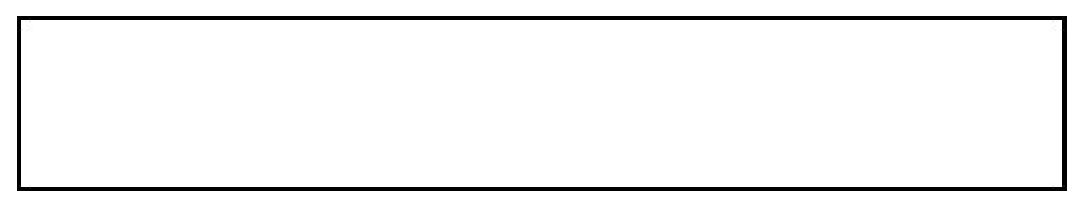
\includegraphics[width=0.9\textwidth]{fig.eps}
\caption{This is a widefig. This is an example of long caption this is an example of long caption  this is an example of long caption this is an example of long caption}\label{fig1}
\end{figure}

In case of double column layout, the above format puts figure captions/images to single column width. To get spanned images, we need to provide \verb+\begin{figure*}+ \verb+...+ \verb+\end{figure*}+.

For sample purpose, we have included the width of images in the optional argument of \verb+\includegraphics+ tag. Please ignore this. 

\section{Algorithms, Program codes and Listings}\label{sec7}

Packages \verb+algorithm+, \verb+algorithmicx+ and \verb+algpseudocode+ are used for setting algorithms in \LaTeX\ using the format:

%%=============================================%%
%% For presentation purpose, we have included  %%
%% \bigskip command. please ignore this.       %%
%%=============================================%%
\bigskip
\begin{verbatim}
\begin{algorithm}
\caption{<alg-caption>}\label{<alg-label>}
\begin{algorithmic}[1]
. . .
\end{algorithmic}
\end{algorithm}
\end{verbatim}
\bigskip
%%=============================================%%
%% For presentation purpose, we have included  %%
%% \bigskip command. please ignore this.       %%
%%=============================================%%

You may refer above listed package documentations for more details before setting \verb+algorithm+ environment. For program codes, the ``program'' package is required and the command to be used is \verb+\begin{program}+ \verb+...+ \verb+\end{program}+. A fast exponentiation procedure:

\begin{program}
\BEGIN \\ %
  \FOR i:=1 \TO 10 \STEP 1 \DO
     |expt|(2,i); \\ |newline|() \OD %
\rcomment{Comments will be set flush to the right margin}
\WHERE
\PROC |expt|(x,n) \BODY
          z:=1;
          \DO \IF n=0 \THEN \EXIT \FI;
             \DO \IF |odd|(n) \THEN \EXIT \FI;
\COMMENT{This is a comment statement};
                n:=n/2; x:=x*x \OD;
             \{ n>0 \};
             n:=n-1; z:=z*x \OD;
          |print|(z) \ENDPROC
\END
\end{program}


\begin{algorithm}
\caption{Calculate $y = x^n$}\label{algo1}
\begin{algorithmic}[1]
\Require $n \geq 0 \vee x \neq 0$
\Ensure $y = x^n$ 
\State $y \Leftarrow 1$
\If{$n < 0$}\label{algln2}
        \State $X \Leftarrow 1 / x$
        \State $N \Leftarrow -n$
\Else
        \State $X \Leftarrow x$
        \State $N \Leftarrow n$
\EndIf
\While{$N \neq 0$}
        \If{$N$ is even}
            \State $X \Leftarrow X \times X$
            \State $N \Leftarrow N / 2$
        \Else[$N$ is odd]
            \State $y \Leftarrow y \times X$
            \State $N \Leftarrow N - 1$
        \EndIf
\EndWhile
\end{algorithmic}
\end{algorithm}
\bigskip
%%=============================================%%
%% For presentation purpose, we have included  %%
%% \bigskip command. please ignore this.       %%
%%=============================================%%

Similarly, for \verb+listings+, use the \verb+listings+ package. \verb+\begin{lstlisting}+ \verb+...+ \verb+\end{lstlisting}+ is used to set environments similar to \verb+verbatim+ environment. Refer to the \verb+lstlisting+ package documentation for more details.

%%=============================================%%
%% For presentation purpose, we have included  %%
%% \bigskip command. please ignore this.       %%
%%=============================================%%
\bigskip
\begin{minipage}{\hsize}%
\lstset{frame=single,framexleftmargin=-1pt,framexrightmargin=-17pt,framesep=12pt,linewidth=0.98\textwidth,language=pascal}% Set your language (you can change the language for each code-block optionally)
%%% Start your code-block
\begin{lstlisting}
for i:=maxint to 0 do
begin
{ do nothing }
end;
Write('Case insensitive ');
Write('Pascal keywords.');
\end{lstlisting}
\end{minipage}

\section{Cross referencing}\label{sec8}

Environments such as figure, table, equation and align can have a label
declared via the \verb+\label{#label}+ command. For figures and table
environments use the \verb+\label{}+ command inside or just
below the \verb+\caption{}+ command. You can then use the
\verb+\ref{#label}+ command to cross-reference them. As an example, consider
the label declared for Figure~\ref{fig1} which is
\verb+\label{fig1}+. To cross-reference it, use the command 
\verb+Figure \ref{fig1}+, for which it comes up as
``Figure~\ref{fig1}''. 

To reference line numbers in an algorithm, consider the label declared for the line number 2 of Algorithm~\ref{algo1} is \verb+\label{algln2}+. To cross-reference it, use the command \verb+\ref{algln2}+ for which it comes up as line~\ref{algln2} of Algorithm~\ref{algo1}.

\subsection{Details on reference citations}\label{subsec7}

Standard \LaTeX\ permits only numerical citations. To support both numerical and author-year citations this template uses \verb+natbib+ \LaTeX\ package. For style guidance please refer to the template user manual.

Here is an example for \verb+\cite{...}+: \cite{bib1}. Another example for \verb+\citep{...}+: \citep{bib2}. For author-year citation mode, \verb+\cite{...}+ prints Jones et al. (1990) and \verb+\citep{...}+ prints (Jones et al., 1990).

All cited bib entries are printed at the end of this article: \cite{bib3}, \cite{bib4}, \cite{bib5}, \cite{bib6}, \cite{bib7}, \cite{bib8}, \cite{bib9}, \cite{bib10}, \cite{bib11} and \cite{bib12}.

\section{Examples for theorem like environments}\label{sec10}

For theorem like environments, we require \verb+amsthm+ package. There are three types of predefined theorem styles exists---\verb+thmstyleone+, \verb+thmstyletwo+ and \verb+thmstylethree+ 

%%=============================================%%
%% For presentation purpose, we have included  %%
%% \bigskip command. please ignore this.       %%
%%=============================================%%
\bigskip
\begin{tabular}{|l|p{19pc}|}
\hline
\verb+thmstyleone+ & Numbered, theorem head in bold font and theorem text in italic style \\\hline
\verb+thmstyletwo+ & Numbered, theorem head in roman font and theorem text in italic style \\\hline
\verb+thmstylethree+ & Numbered, theorem head in bold font and theorem text in roman style \\\hline
\end{tabular}
\bigskip

\noindent
For a quote environment, use \verb+\begin{quote}...\end{quote}+
\begin{quote}
Quoted text example. Aliquam porttitor quam a lacus. Praesent vel arcu ut tortor cursus volutpat. In vitae pede quis diam bibendum placerat. Fusce elementum
convallis neque. Sed dolor orci, scelerisque ac, dapibus nec, ultricies ut, mi. Duis nec dui quis leo sagittis commodo.
\end{quote}

Sample body text. Sample body text. Sample body text. Sample body text. Sample body text (refer Figure~\ref{fig1}). Sample body text. Sample body text. Sample body text (refer Table~\ref{tab3}). 

\section{Methods}\label{sec11}

Topical subheadings are allowed. Authors must ensure that their Methods section includes adequate experimental and characterization data necessary for others in the field to reproduce their work. Authors are encouraged to include RIIDs where appropriate. 

\textbf{Ethical approval declarations} (only required where applicable) Any article reporting experiment/s carried out on (i)~live vertebrate (or higher invertebrates), (ii)~humans or (iii)~human samples must include an unambiguous statement within the methods section that meets the following requirements: 

\begin{enumerate}[1.]
\item Approval: a statement which confirms that all experimental protocols were approved by a named institutional and/or licensing committee. Please identify the approving body in the methods section

\item Accordance: a statement explicitly saying that the methods were carried out in accordance with the relevant guidelines and regulations

\item Informed consent (for experiments involving humans or human tissue samples): include a statement confirming that informed consent was obtained from all participants and/or their legal guardian/s
\end{enumerate}

If your manuscript includes potentially identifying patient/participant information, or if it describes human transplantation research, or if it reports results of a clinical trial then  additional information will be required. Please visit (\url{https://www.nature.com/nature-research/editorial-policies}) for Nature Portfolio journals, (\url{https://www.springer.com/gp/authors-editors/journal-author/journal-author-helpdesk/publishing-ethics/14214}) for Springer Nature journals, or (\url{https://www.biomedcentral.com/getpublished/editorial-policies\#ethics+and+consent}) for BMC.

\section{Discussion}\label{sec12}

Discussions should be brief and focused. In some disciplines use of Discussion or `Conclusion' is interchangeable. It is not mandatory to use both. Some journals prefer a section `Results and Discussion' followed by a section `Conclusion'. Please refer to Journal-level guidance for any specific requirements. 

\section{Conclusion}\label{sec13}

Conclusions may be used to restate your hypothesis or research question, restate your major findings, explain the relevance and the added value of your work, highlight any limitations of your study, describe future directions for research and recommendations. 

In some disciplines use of Discussion or 'Conclusion' is interchangeable. It is not mandatory to use both. Please refer to Journal-level guidance for any specific requirements. 

\backmatter

\bmhead{Supplementary information}

If your article has accompanying supplementary file/s please state so here. 

Authors reporting data from electrophoretic gels and blots should supply the full unprocessed scans for key as part of their Supplementary information. This may be requested by the editorial team/s if it is missing.

Please refer to Journal-level guidance for any specific requirements.

\bmhead{Acknowledgments}

Acknowledgments are not compulsory. Where included they should be brief. Grant or contribution numbers may be acknowledged.

Please refer to Journal-level guidance for any specific requirements.

\section*{Declarations}

Some journals require declarations to be submitted in a standardised format. Please check the Instructions for Authors of the journal to which you are submitting to see if you need to complete this section. If yes, your manuscript must contain the following sections under the heading `Declarations':

\begin{itemize}
\item Funding
\item Conflict of interest/Competing interests (check journal-specific guidelines for which heading to use)
\item Ethics approval 
\item Consent to participate
\item Consent for publication
\item Availability of data and materials
\item Code availability 
\item Authors' contributions
\end{itemize}

\noindent
If any of the sections are not relevant to your manuscript, please include the heading and write `Not applicable' for that section. 

%%===================================================%%
%% For presentation purpose, we have included        %%
%% \bigskip command. please ignore this.             %%
%%===================================================%%
\bigskip
\begin{flushleft}%
Editorial Policies for:

\bigskip\noindent
Springer journals and proceedings: \url{https://www.springer.com/gp/editorial-policies}

\bigskip\noindent
Nature Portfolio journals: \url{https://www.nature.com/nature-research/editorial-policies}

\bigskip\noindent
\textit{Scientific Reports}: \url{https://www.nature.com/srep/journal-policies/editorial-policies}

\bigskip\noindent
BMC journals: \url{https://www.biomedcentral.com/getpublished/editorial-policies}
\end{flushleft}

\begin{appendices}

\section{Section title of first appendix}\label{secA1}

An appendix contains supplementary information that is not an essential part of the text itself but which may be helpful in providing a more comprehensive understanding of the research problem or it is information that is too cumbersome to be included in the body of the paper.

%%=============================================%%
%% For submissions to Nature Portfolio Journals %%
%% please use the heading ``Extended Data''.   %%
%%=============================================%%

%%=============================================================%%
%% Sample for another appendix section			       %%
%%=============================================================%%

%% \section{Example of another appendix section}\label{secA2}%
%% Appendices may be used for helpful, supporting or essential material that would otherwise 
%% clutter, break up or be distracting to the text. Appendices can consist of sections, figures, 
%% tables and equations etc.

\end{appendices}

%%===========================================================================================%%
%% If you are submitting to one of the Nature Portfolio journals, using the eJP submission   %%
%% system, please include the references within the manuscript file itself. You may do this  %%
%% by copying the reference list from your .bbl file, paste it into the main manuscript .tex %%
%% file, and delete the associated \verb+\bibliography+ commands.                            %%
%%===========================================================================================%%

\bibliographystyle{bst/sn-basic}
\bibliography{sn-bibliography}% common bib file
%% if required, the content of .bbl file can be included here once bbl is generated
%%\input sn-article.bbl

%% Default %%
%%\input sn-sample-bib.tex%

\end{document}
